\documentclass{scrartcl}

% Bibliography Preamble
\usepackage[backend=biber,style=apa,sorting=none]{biblatex}
\addbibresource{Design-Document.bib}
\let\cite\textcite
\let\citep\autocite

% Graphic / Figure Preamble
\usepackage{graphicx}
\graphicspath{{img/}}

\usepackage{hyperref}

\begin{document}
\author{Charlotte Ward}
\title{ {\huge Cybersky - Design Document} \\ {\small Shoot 'Em Up Game} }
\maketitle

\section{Game Rules}

\subsection{Basis}

\subsubsection{Space Invaders (1978)}

\begin{figure}[ht]
  \centering
  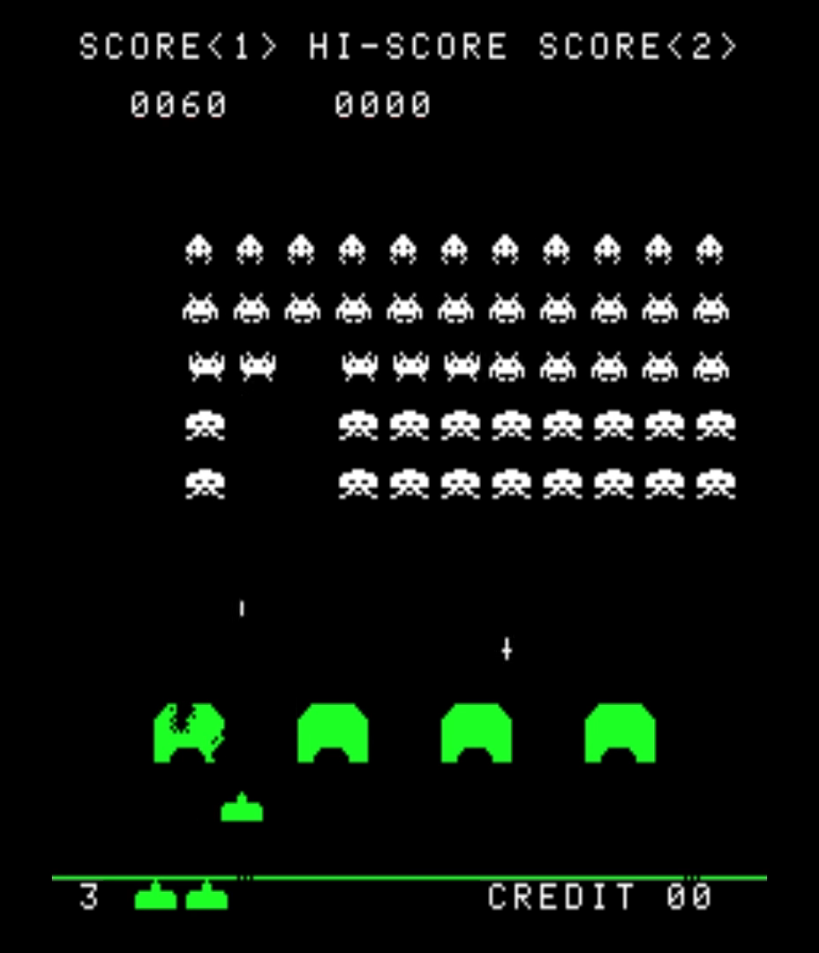
\includegraphics[width=.35\columnwidth]{SpaceInvaders.png}
  \caption[\textit{Space Invaders}]{\textit{Space Invaders} (1978) Gameplay Still from \cite{Youtube001}}
\end{figure}

Released in 1978 as an Arcade game, only 6 years after the initial release of \textit{PONG}, \textit{Space Invaders} pionered the genre of Fixed Shooter games in the arcade form factor, later becoming the basis for Shoot 'Em Up games. With the arcade game industry going through something of a 'Golden Age' \citep{BMIGaming001}, \textit{Space Invaders} was at the forefront of the industry's growth, reaching number 2 of all time in terms of sales and revenue \citep{USGamer001}.

With Shoot 'Em Up games mimicing many of the features and game rules utilised by \textit{Space Invaders}, it's important to take a look back and see exactly how the game worked and what the source of it's popularity is.

\begin{figure}[ht]
  \centering
  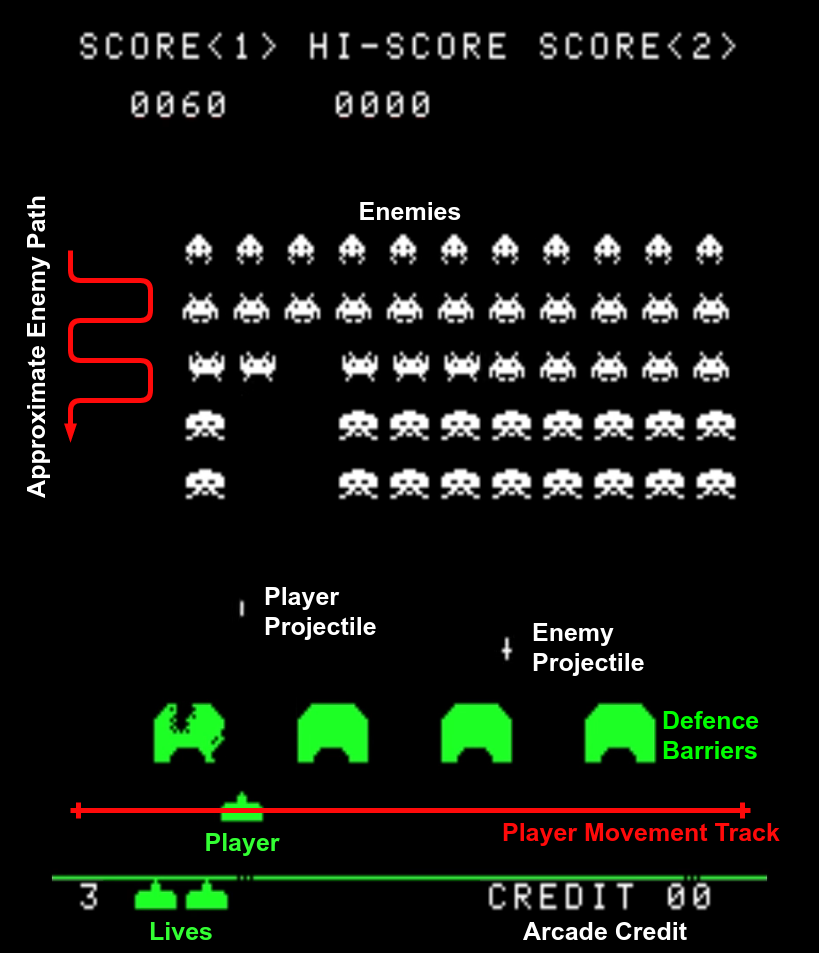
\includegraphics[width=.6\columnwidth]{SpaceInvadersBreakdown.png}
  \caption[\textit{Space Invaders}]{Modified \textit{Space Invaders} (1978) Gameplay Still from \cite{Youtube001}}
\end{figure}

This figure annotates some of the core elements in the gameplay of \textit{Space Invaders}. These elements will become important moving forward, as the Shoot 'Em Up (hereby referred to as Shmup) genre develops alongside games as a whole. These key points include:

\begin{itemize}
  \item The player can move from left to right, using an invisible track to dictate the bounds of movement.
  \item The player can fire projectiles from their player object, which fly upwards and don't move horizontally. When they hit an enemy that enemy is destroyed, and the score increments upwards.
  \item The enemies are grouped together, and follow a set path. At certain intervals, they fire projectiles towards the player, which must be avoided. Failure to avoid a projectile results in losing a life.
  \item There are barriers which can block player or enemy projectiles, but are damaged whenever they do. They can be removed completely with enough projectiles.
\end{itemize}

\subsubsection{Galaxian (1979)}

\begin{figure}[ht]
  \centering
  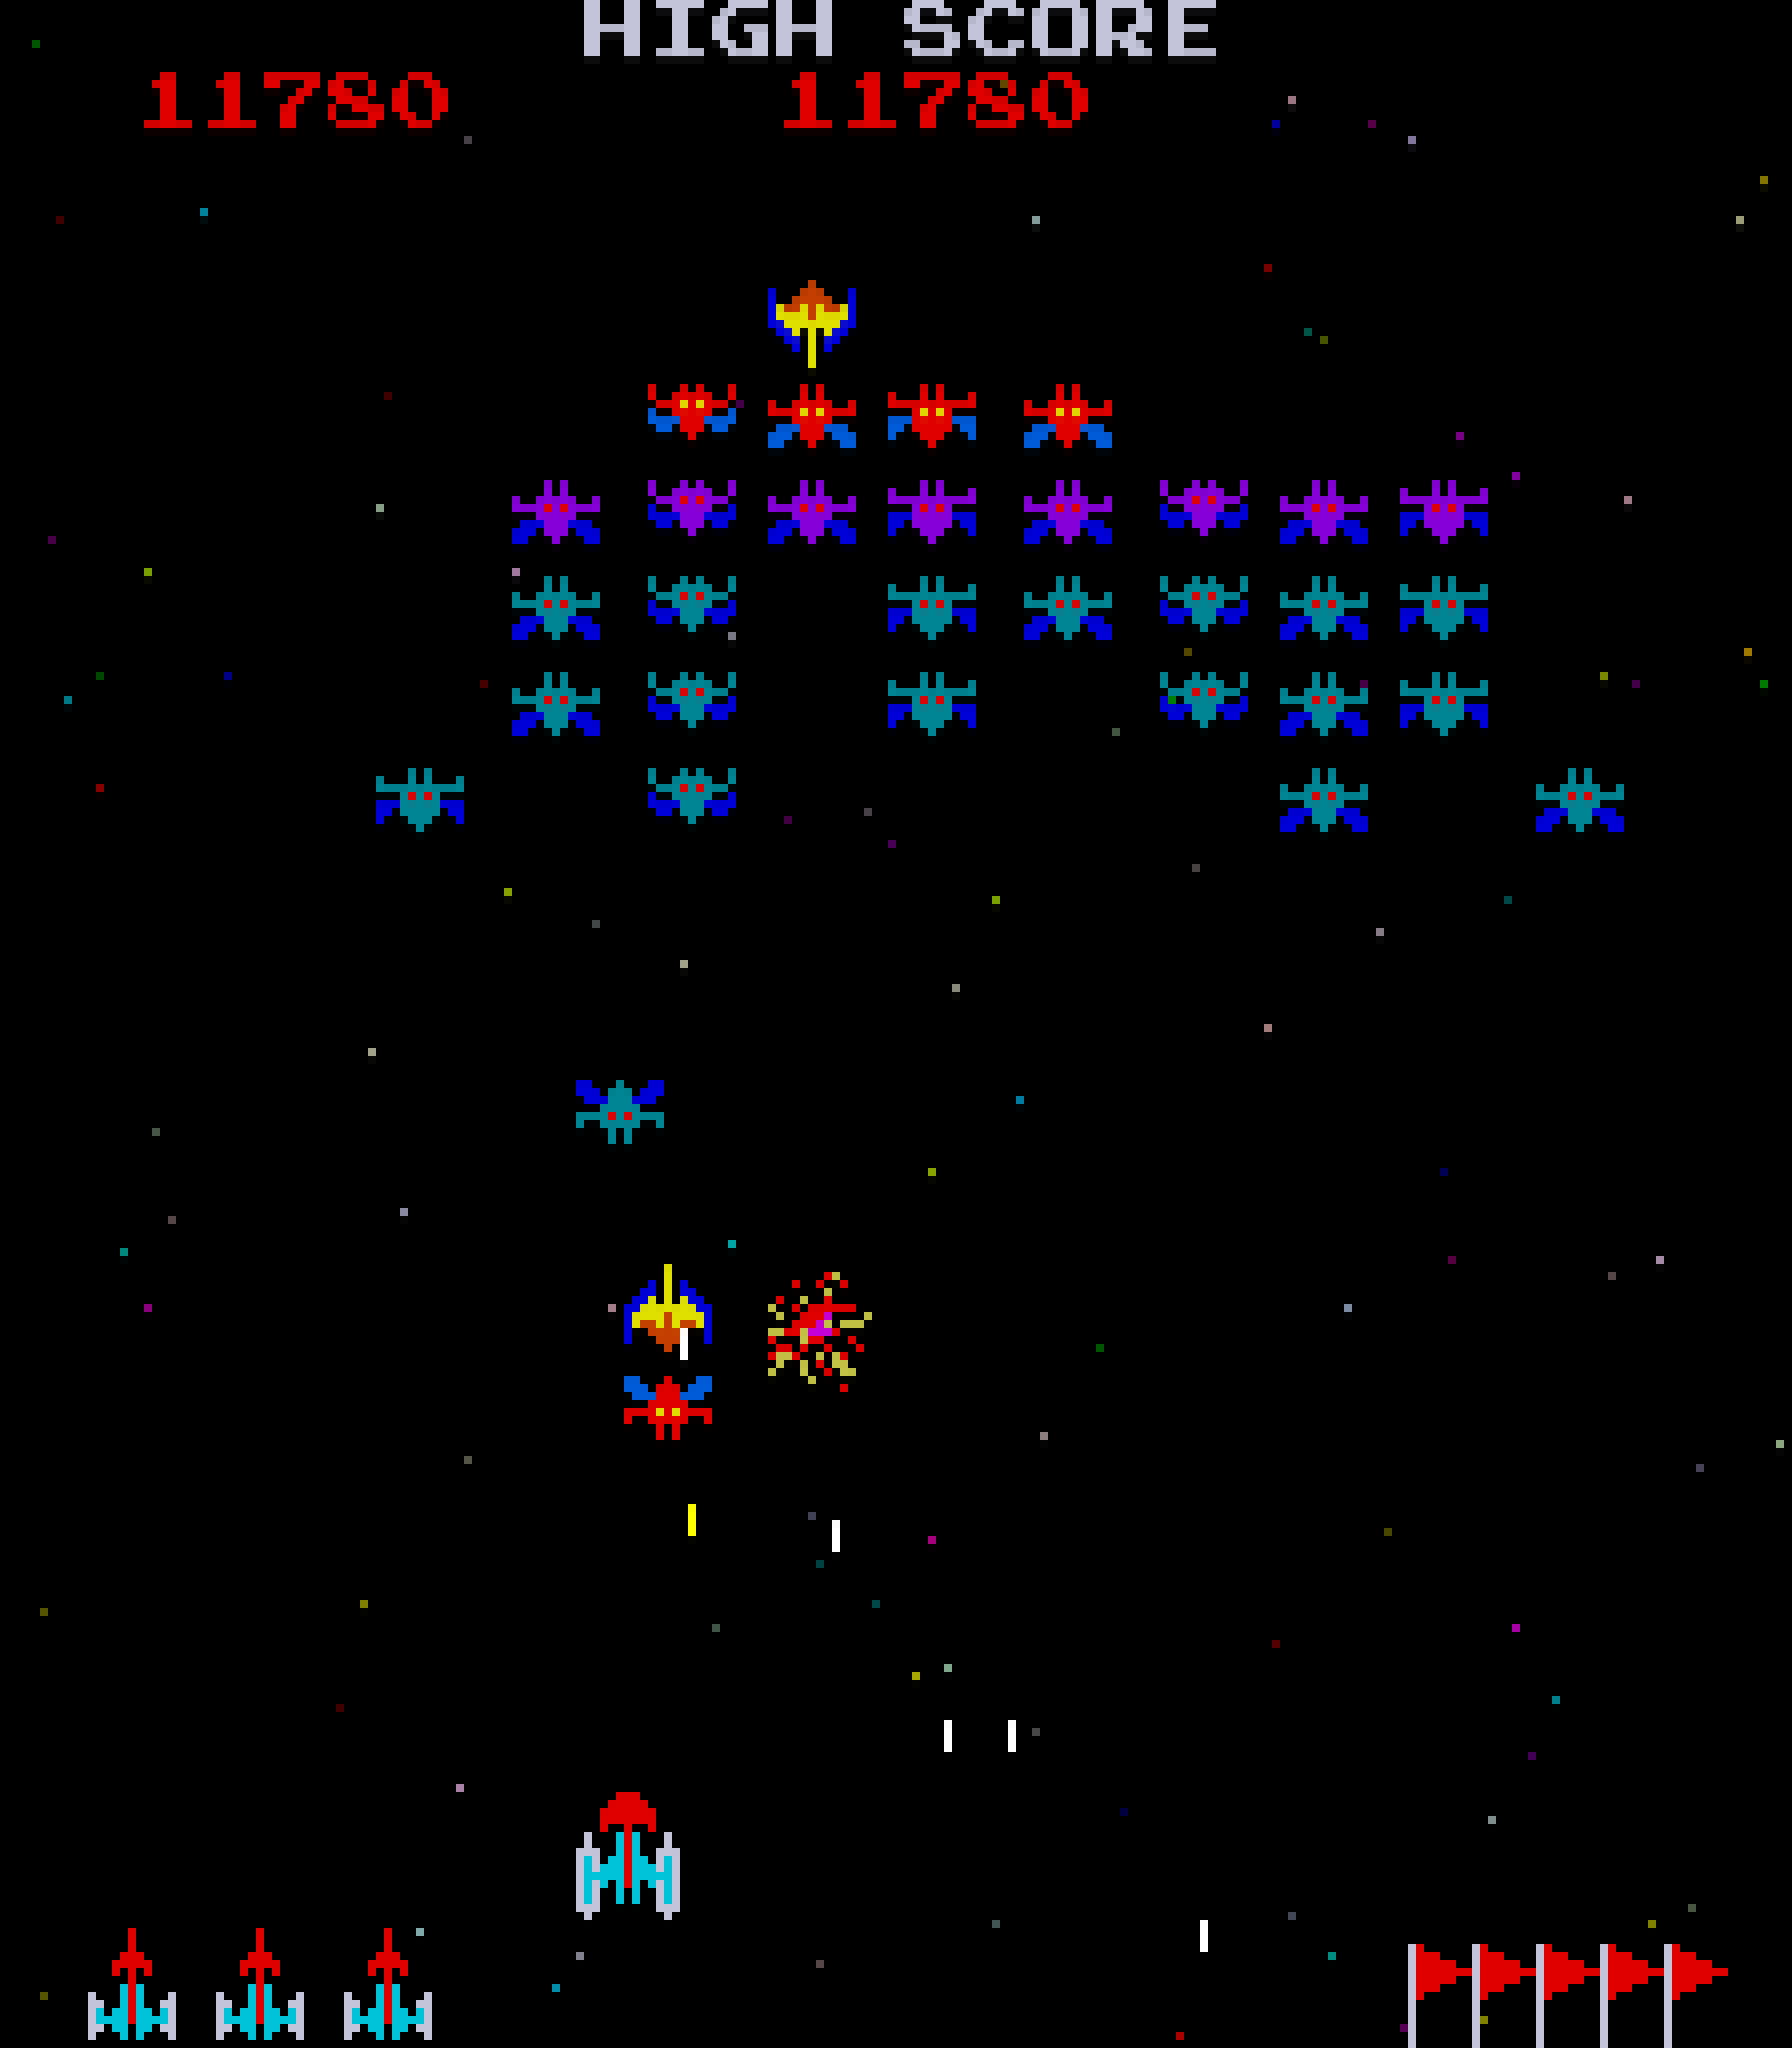
\includegraphics[width=.6\columnwidth]{Galaxian.png}
  \caption[\textit{Galaxian}]{\textit{Galaxian} (1979) Gameplay Still by \cite{Wikimedia001}}
\end{figure}


Released only a year after \textit{Space Invaders}, \textit{Galaxian} (1979) further extends the Fixed Shooter genre, improving upon \textit{Space Invader}'s successes; many of the core features remain the same, with a large group of enemies at the top of the screen, and a fixed track for player movement. The projectile system remains the same additionally, with both the player's projectiles and enemy projectiles functioning similarly.

The main differences between the two games come from differences in the visual design, gameplay complexity and overall changes in the arcade cabinet itself \citep{Youtube002}. While it's difficult to directly compare the hardware included in arcade cabinets, it's clear that the complexity involved in the game \textit{Galaxian} far outweighs that of \textit{Space Invaders}:

\begin{itemize}
  \item \textit{Galaxian} has an improved colour screen, with multi-coloured sprites.
  \item The game features a scrolling background with stars that sparkle.
  \item Enemies have animated sprites, improving on \textit{Space Invader}'s simple sprites.
\end{itemize}

The gameplay revolves around an endless mode, where there's no set amount of enemies. As 'waves' of enemies are defeated, new waves turn up afterwards. This kind of gameplay is somewhat cyclical, with the core gameplay loop involving defeating batches of enemies, then progressing onto a new batch.

Additionally, the individual 'aliens' that show up in a wave can break off and fly towards the player, firing projectiles at the same time. The gameplay becomes much more hectic because of this, with many things happening on screen at once. This is an improvement on Space Invaders, where very little may be happening in a given moment.

\subsubsection{Ikaruga (2001)}

\begin{figure}[ht]
  \centering
  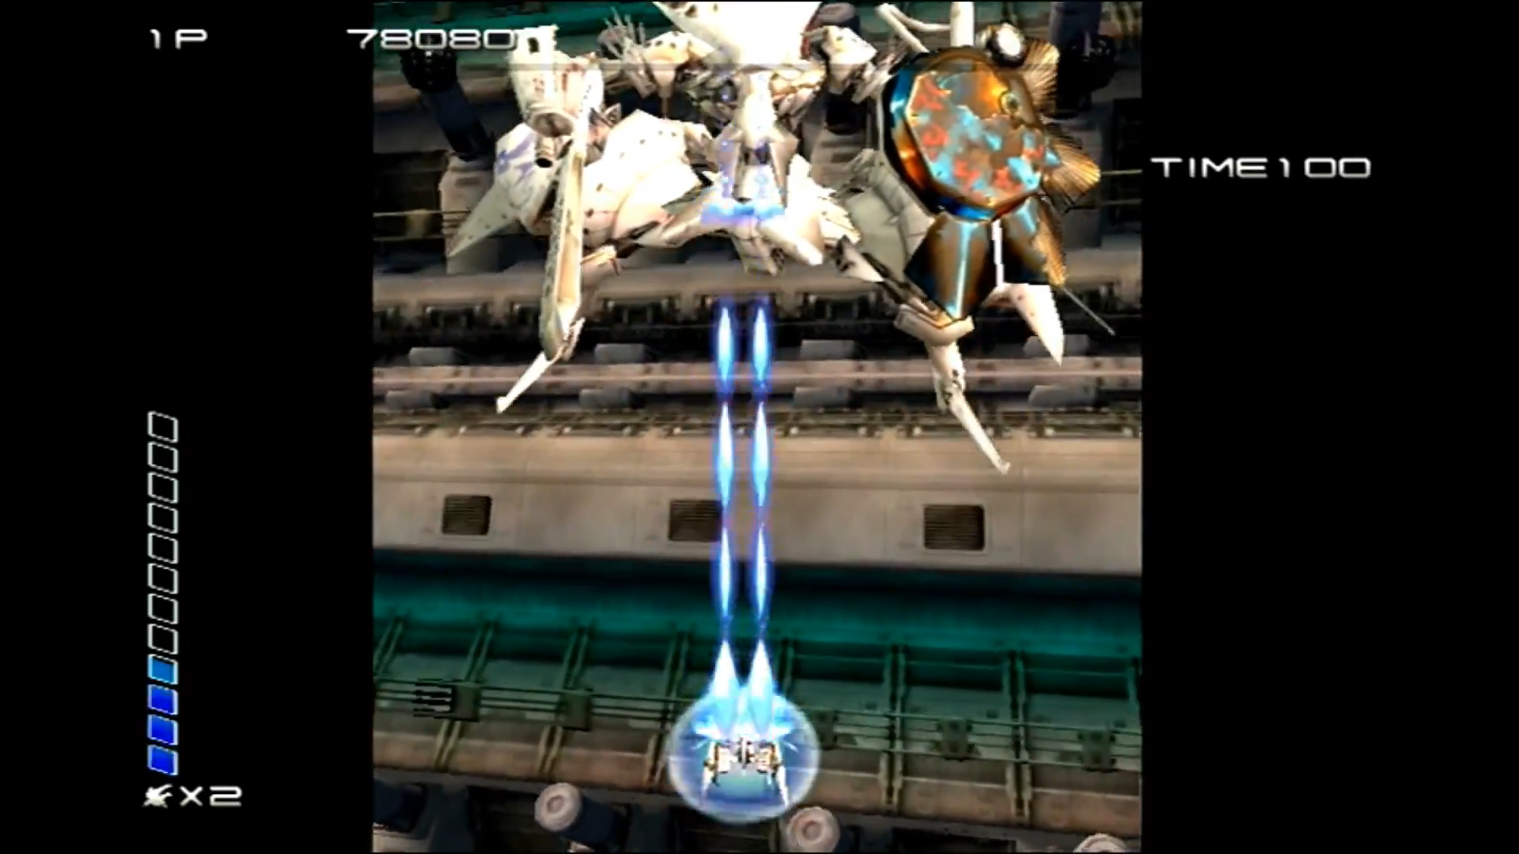
\includegraphics[width=.7\columnwidth]{Ikaruga.png}
  \caption[\textit{Ikaruga}]{\textit{Ikaruga} (2001) Gameplay Still by \cite{Youtube003}}
\end{figure}

Skipping forward a few decades, \textit{Ikaruga}, originally released in 2001, expands further upon the established gameplay rules for Shmups, with clear inspiration taken from Galaxian in the implementation of movement systems and overall gameplay. The game itself recieved a moderate following, finding the most success as a cult classic within the Bullet Hell fandom, being widely regarded as one of the best Shmups available \citep{GiantBomb002}.

While it's true that the average scene in \textit{Ikaruga} has far more going on, staying true to the moniker of Bullet Hell, both games are still relatively similar. If you boil the two games down to their core elements, not much has changed. The primary differences relate to the movement system that the player has, as well as some extra mechanical depth that comes from a toggle that the player can use.

The movement system in \textit{Ikaruga} is two dimensional, allowing the player to move forward and backward as well as left and right. I believe that the reasoning behind this relates to the player's ability to dodge attacks, making the positioning that the player can utilise much more interesting and deep by literally adding another dimension to it.

The other main mechanic used by \textit{Ikaruga} is a toggle that switches the player between a 'light mode' and a 'dark mode'. This is a mechanic that's mirrored in the gameplay scene, with attacks coming from enemies fitting into one of these two groups. This mechanic allows for the player to have additional control over the scene, letting them choose which kind of attack to avoid or intercept.

\subsection{Design}

\subsubsection{Controls}

With the historical basis of Shmups in mind, it's clear that a few elements fit in quite well with the overall structure of a mobile game. All of the games explored feature a display that is taller than it is wide, which lends itself well to the form factor that a mobile phone has. Additionally, they retain simple-yet-complex mechanics for movement and interaction, which fits very well with the more simple interface of a touch-screen. Using this knowledge, it's possible to design a simple wireframe version of the game \textit{Cybersky}.

\begin{figure}[ht]
  \centering
  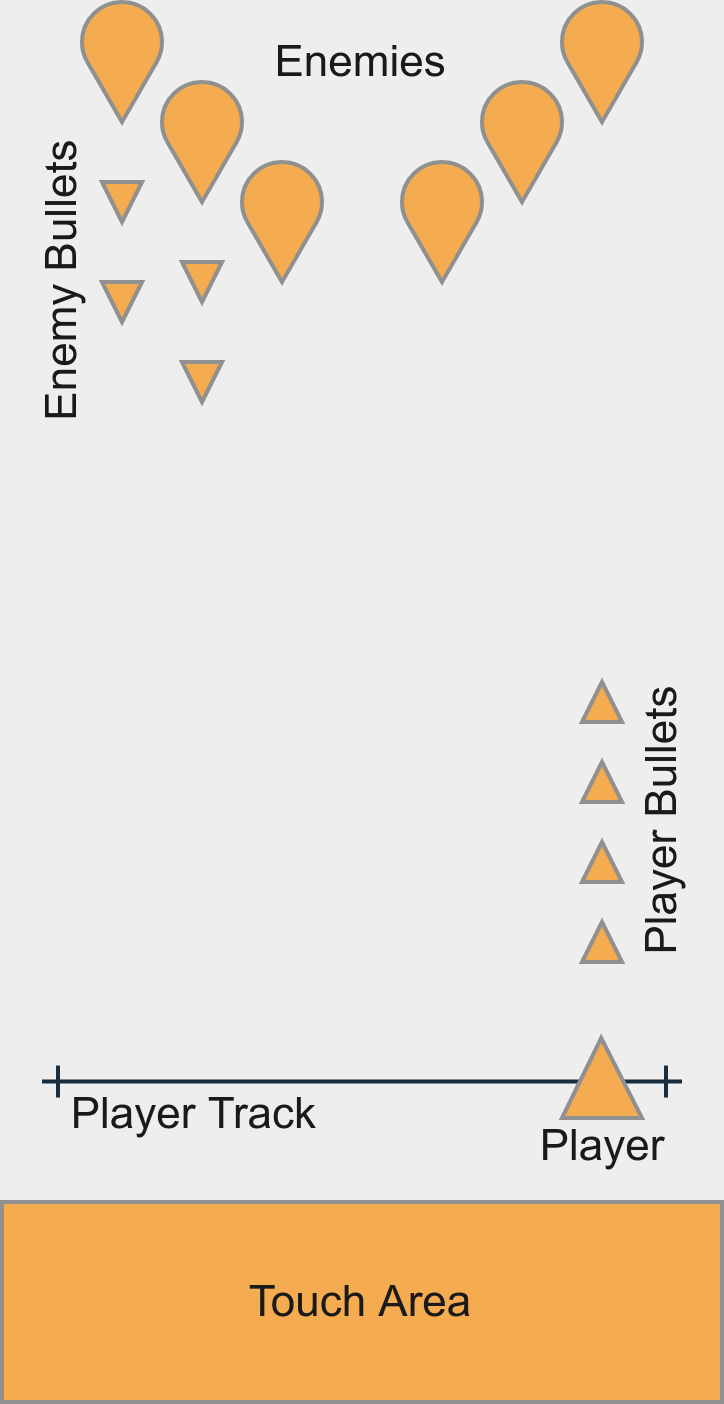
\includegraphics[width=.3\columnwidth]{concept1.png}
  \caption[\textit{Cybersky}]{\textit{Cybersky} Scene Wireframe}
\end{figure}

Figure 5 illustrates the overall design concept, showing the player on a track allowing for horizontal movement, as well as the bullets that the player can fire. Additionally, it shows a small set of enemies at the top of the screen. Borrowing elements from \textit{Galaxian} and \textit{Ikaruga}, I'd like for the player to have to dodge enemies, using the touch area at the bottom of the screen to control the horizontal position of the player element.

\begin{figure}[ht]
  \centering
  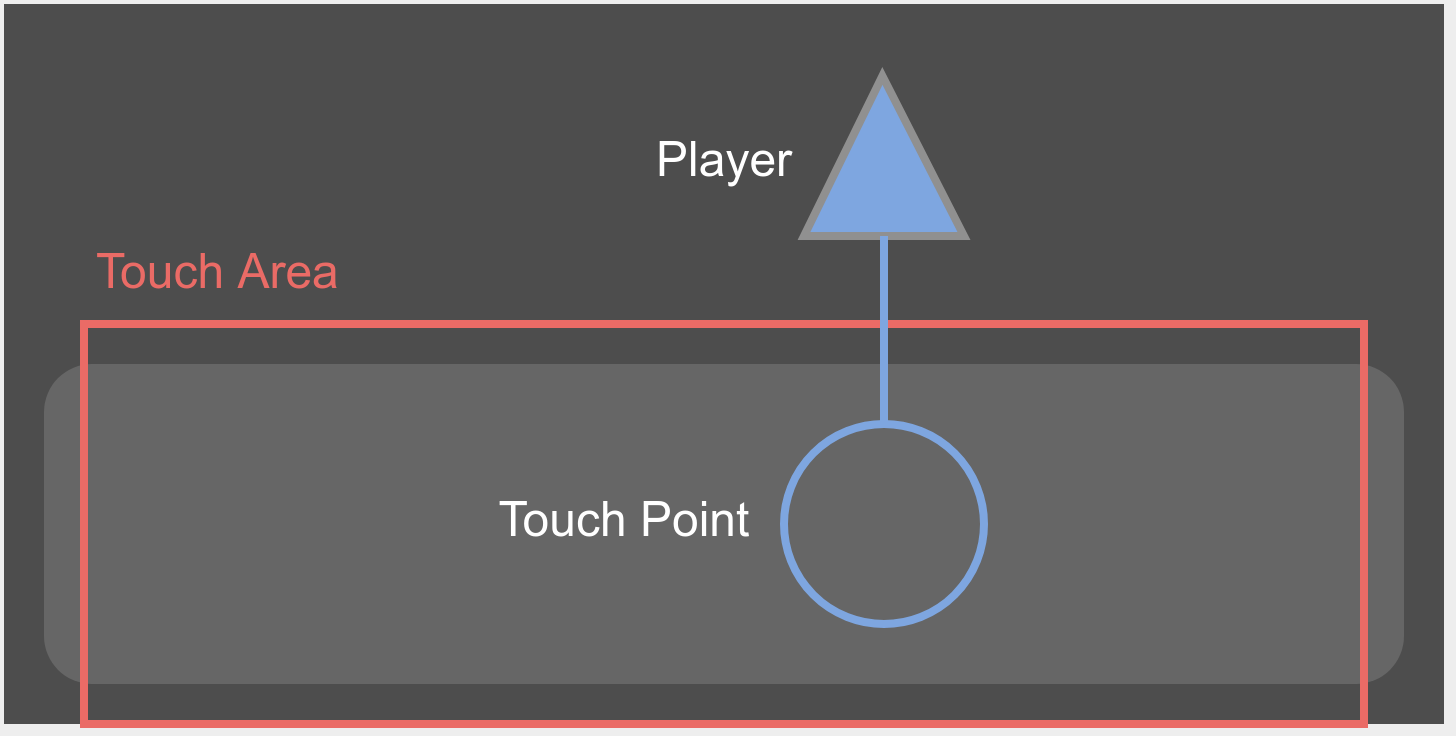
\includegraphics[width=.6\columnwidth]{concept4.png}
  \caption[\textit{Cybersky}]{\textit{Cybersky} Scene Wireframe showing Touch Input}
\end{figure}

Using the touch area at the bottom of the screen to control horizontal movement would involve having the player element follow where the touch point is. This allows for the player to swipe along the bottom of the screen to move horizontally. Doing some rudimentary testing on my own phone, I feel as though this provides a fair amount of control, as swiping in this area is fairly easy.

\subsubsection{Enemies}

My vision for the enemies in this game mirror what's implemented in \textit{Ikaruga}, and many similar games in other genres, splitting the enemy pool into three major categories.

\begin{itemize}

  \item Fodder - Designed to fill out the screen and give the player something to avoid and shoot and dodge. Usually these appear in groups.
  \item Special - Ranges in health and difficulty, but with some kind of gimmick.

  \item Larger Enemies - Take more hits to destroy, more of a threat.

  \item Boss - Large enemies that take up one side of the screen. These enemies usually have distinct phases and gimmicks. A basic example of this would be a boss that flips the screen. Each boss would require the player to overcome said gimmick in order to effectively fight it.
  \item End-Boss - Similar in scale and difficulty to a regular boss, but usually the end-game bosses recycle gimmicks and phases. Probably best to make this more of a bullet hell than the rest of the bosses.

\end{itemize}


\section{Target Audience}

\subsection{Group 1 - Shmup and Hardcore Gamers}

As Shmups are fairly niche, with a complex and storied history, I feel that catering primarily to fans of the genre, and those that consider themselves 'hardcore' gamers, would be a good starting point for this game.

Reaching this kind of player may be more difficult than it seems, as mobile games tend to have a very negative reputation with gamers \citep{AndroidAuthority001}. This comes, primarily, from the perception that mobile games are pointless, have no content, and try to steal ideas from other games in order to boil them down into a product. Having a mobile game that stays true to the origins of the Shmup genre may be key to winning over this demographic.

\subsection{Group 2 - Commuters and Casual Gamers}

As this is a mobile game, consideration should be placed onto the wider market of more casual users. Commuters are an ideal focus for this, as they're the ideal example of a casual player of someone who has engages in shorter play sessions, namely during a commute, and perhaps doesn't want to focus on difficult gameplay or hard enemies.

According to \cite{Verto001}, the average gamer only spends 24 minutes a day playing mobile games, reflecting the shorter time allowance afforded by commuting and day-to-day free time. Mobile games, in this instance, are used to fill time in someone's day where otherwise they may be doing nothing.

This is the core market of mobile games, with the success of a mobile game being reliant somewhat on the session time, and the ease of access for a game. Shorter session times can materially impact player retention, which has knock-on effects with the success of the game.

\section{Scoring}

\subsection{Game Modes}

\subsubsection{Story}

A story mode for a shmup typically has segmented levels that all fall under 'chapters', which all have unique themes and introduce mechanics. This level system allows for chapters and their sublevels to gain ratings based on the score you get in each level.

Influenced by the earlier described arcade games, shmups in today's market tend to borrow the scoring systems used, involving a simple points system for damaging and destroying enemies. While there's many ways for this to get more mechanically complex. There are a few examples of this being implemented in the games above, although it would be interesting to further iterate on this idea.

Borrowing from this game mode archetype, I think it'd be interesting to have a light 'story' mode in my game, perhaps skipping the more narrative-focussed elements that usually come along with a story, instead utilising the framework for aesthetic and difficulty progression. Additionally, this could make the game more accessible to mobile users, as shorter bursts of gameplay tend to be more appreciated on the mobile market \citep{Verto001}.

On top of this, having a hi-score system for each level, chapter, and the story as a whole may add a kind of scoring progression, making the player feel better about working harder and meeting a new high.

\subsubsection{Endless}

As well as a 'story' mode, having an Endless mode could be appealing for some users, with a steady progression of difficulty over time rather than over levels. This also makes it easier for users to pick up and play, as it's a fast track into more engaging gameplay than a story mode, which may have the player stuck in an easier level, and also is much easier to put down as there's no pressure of finishing the level they're on.

This kind of game mode relies on scoring, with a stopwatch and a ticking scorebar being integral to the progression of any endless mode. There's room here for improvement, additionally, such as a customiseable endless mode, a challenge mode, and some gameplay progression inside the mode that mirrors the episodic nature of the story mode, like with phases. Further exploration of this idea should focus around user requirements.

\section{Reward Mechanics}

\subsection{Customisation}

A core part of reward mechanics involves progression. Having the progression afforded by the story and endless mode, including scoring, is fine, however having a more concrete and tangible unlock system could greatly improve the reward system in-game, and increase engagement. This mechanic is multifaceted, with the potential for both aesthetic and gameplay unlocks.

In the aesthetic paradigm, having unlockable cosmetics is a tried and tested method for engaging the player. It gives them the ability to personalise and customise. As well as this, it clearly illustrates a path of progression, giving them a goal to collect cosmetics. Cosmetics also have an interesting history, with whole economies springing up around the trade and sale of cosmetic items \citep{GamaSutra001}.

On top of this, implementing a loadout system that allows for users to swap out parts of their character would be key, as this could allow for them to customise how they play on top of the aesthetic customisation that comes from cosmetics. Additionally, this could allow for different play styles. For example, swapping out weapons could impact the area of effect, damage type, speed, et cetera. Finally, this would allow for progression in terms of item unlocks, allowing for the player to unlock new equipment and even better equipment. I feel as though progression like this would be perfect for a reward mechanic in this game.

\printbibliography

\end{document}
